\section{Tangentialvektoren und Geschwindigkeit}
Betrachten Sie noch einmal die vier robotergesteuerte Fahrzeuge:
\[
F_1 : \begin{pmatrix}
    x \\y
\end{pmatrix}
 = 
 \begin{pmatrix}
    -8 + 4t \\
 2t
 \end{pmatrix}
\quad
F_2 : \begin{pmatrix}
    x \\y
\end{pmatrix}
 = \begin{pmatrix}
10 - 2t \\
-6 + t
\end{pmatrix}
\quad
F_3 : \begin{pmatrix}
    x \\y
\end{pmatrix}
 = 
 \begin{pmatrix}
    2 \cos\left(\frac{\pi}{4}t\right) \\
    2 \sin\left(\frac{\pi}{4}t\right)
 \end{pmatrix}
 \quad
F_4 : \begin{pmatrix}
    x \\y
\end{pmatrix}
 = \begin{pmatrix}
t \\
\frac{t^2}{4}
\end{pmatrix}
\]
\begin{center}

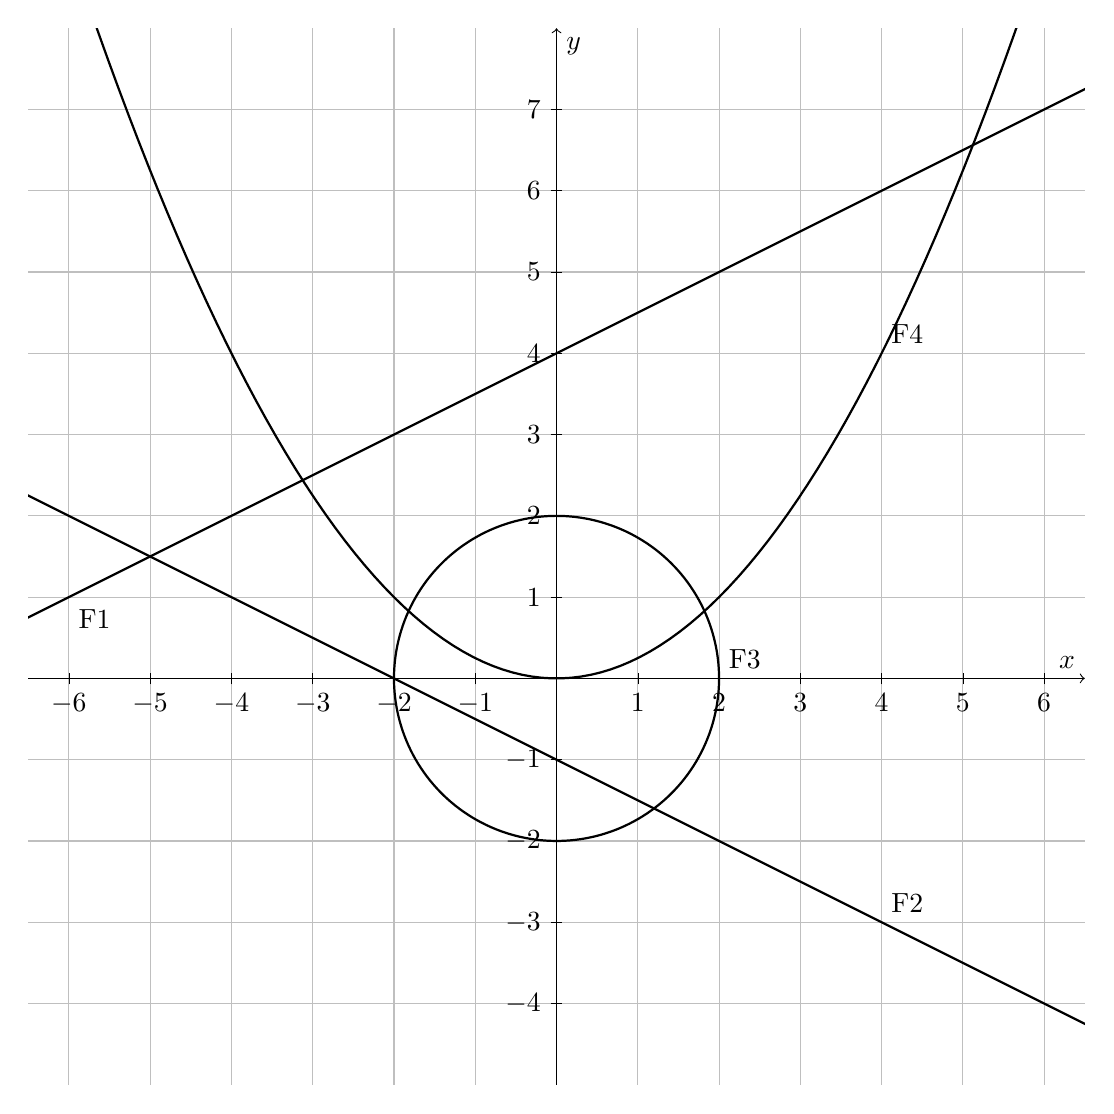
\begin{tikzpicture}
    \begin{axis}[
        grid=both,
        xmin=-6.5, xmax=6.5,
        ymin=-4.5, ymax=7.5,
        axis lines=middle,
        xlabel={$x$},
        ylabel={$y$},
        xtick={-6, -5, ..., 6},
        ytick={-4, -3, ..., 7},
        width=15cm, height=15cm,
        enlargelimits=false,
        axis equal,
        axis line style={->},
        tick style={color=black}
    ]

    % F1
    \addplot[
        domain=0:4, 
        samples=100, 
        thick,
        mark=none
    ] ({-8+4*x}, {2*x});
    \node at (axis cs:-6, 0.5) [anchor=south west] {F1};
    
    % F2
    \addplot[
        domain=0:10, 
        samples=100, 
        thick,
        mark=none
    ] ({10 - 2*x}, {-6 +x});
    \node at (axis cs:4, -3) [anchor=south west] {F2};

    % F3
    \addplot[
        domain=0:2*pi, 
        samples=200, 
        thick,
        mark=none
    ] ({2*cos(deg(x))}, {2*sin(deg(x))});
    \node at (axis cs:2, 0) [anchor=south west] {F3};
    
    % F4
    \addplot[
        domain=-6:6, 
        samples=100, 
        thick,
        mark=none
    ] ({x}, {x^2 / 4});
    \node at (axis cs:4, 4) [anchor=south west] {F4};

    \end{axis}

\end{tikzpicture}
\end{center}
\begin{enumerate}
    \item Ermitteln Sie die Geschwindigkeit der Fahrzeuge.
    \item Sind die Fahrzeuge beschleunigt?
\end{enumerate}

\clearpage

\begin{definition}
    {}{}
            Sei \( \vec{r} \) eine parametrisierte Kurve der Form
        \[
        \vec{r}: \mathbb{R} \to \mathbb{R}^2, \quad t \mapsto \vec{r}(t) = \begin{pmatrix}
        x(t) \\
        y(t)
        \end{pmatrix}
        \]
        Die Ableitung
        \[
        \dot{\vec{r}}: \mathbb{R} \to \mathbb{R}^2, \quad t \mapsto \dot{\vec{r}}(t) = \begin{pmatrix}
        \dot{x}(t) \\
        \dot{y}(t)
        \end{pmatrix}
        \]
        beschreibt den Tangentialvektor der Kurve im Punkt \( r(t) \).

        Wenn man \( \vec{r}(t) \) als den Ortsvektor eines bewegten Objektes zur Zeit \( t \) auffasst, entspricht die Ableitung \( \dot{\vec{r}}(t) \) dem momentanen Geschwindigkeitsvektor \( \vec{v}(t) \) des bewegten Objektes. 

        Die skalare Grösse, die man umgangssprachlich mit Geschwindigkeit bezeichnet, wird \emph{Schnelligkeit} genannt und ist der Betrag des Geschwindigkeitsvektors: \( |\dot{\vec{r}}(t)| = |\vec{v}(t)| \).

        Die Ableitung der Geschwindigkeit ist 
        \[
        \ddot{\vec{r}}: \mathbb{R} \to \mathbb{R}^2, \quad t \mapsto \ddot{\vec{r}}(t) = \begin{pmatrix}
        \ddot{x}(t) \\
        \ddot{y}(t)
        \end{pmatrix}
        \]
        Sie entspricht dem momentanen Beschleunigungsvektor \( \vec{a}(t) \).

        Man beachte: Wenn die unabhängige Variable $t$ ist, wird für die Ableitung in der Regel die Notation $\dot r$ anstatt $r'$ verwendet.

        
\end{definition}

Den Geschwindigkeitsvektor $\dot{\vec{r}}(t)$ interpretiert man in der Regel als Vektor, der am Kurvenpunkt mit Ortsvektor $\vec{r}(t)$ sitzt und von dort in die momentane Bewegungsrichtung zeigt. Seine Länge entspricht der momentanen Schnelligkeit.
\begin{center}
    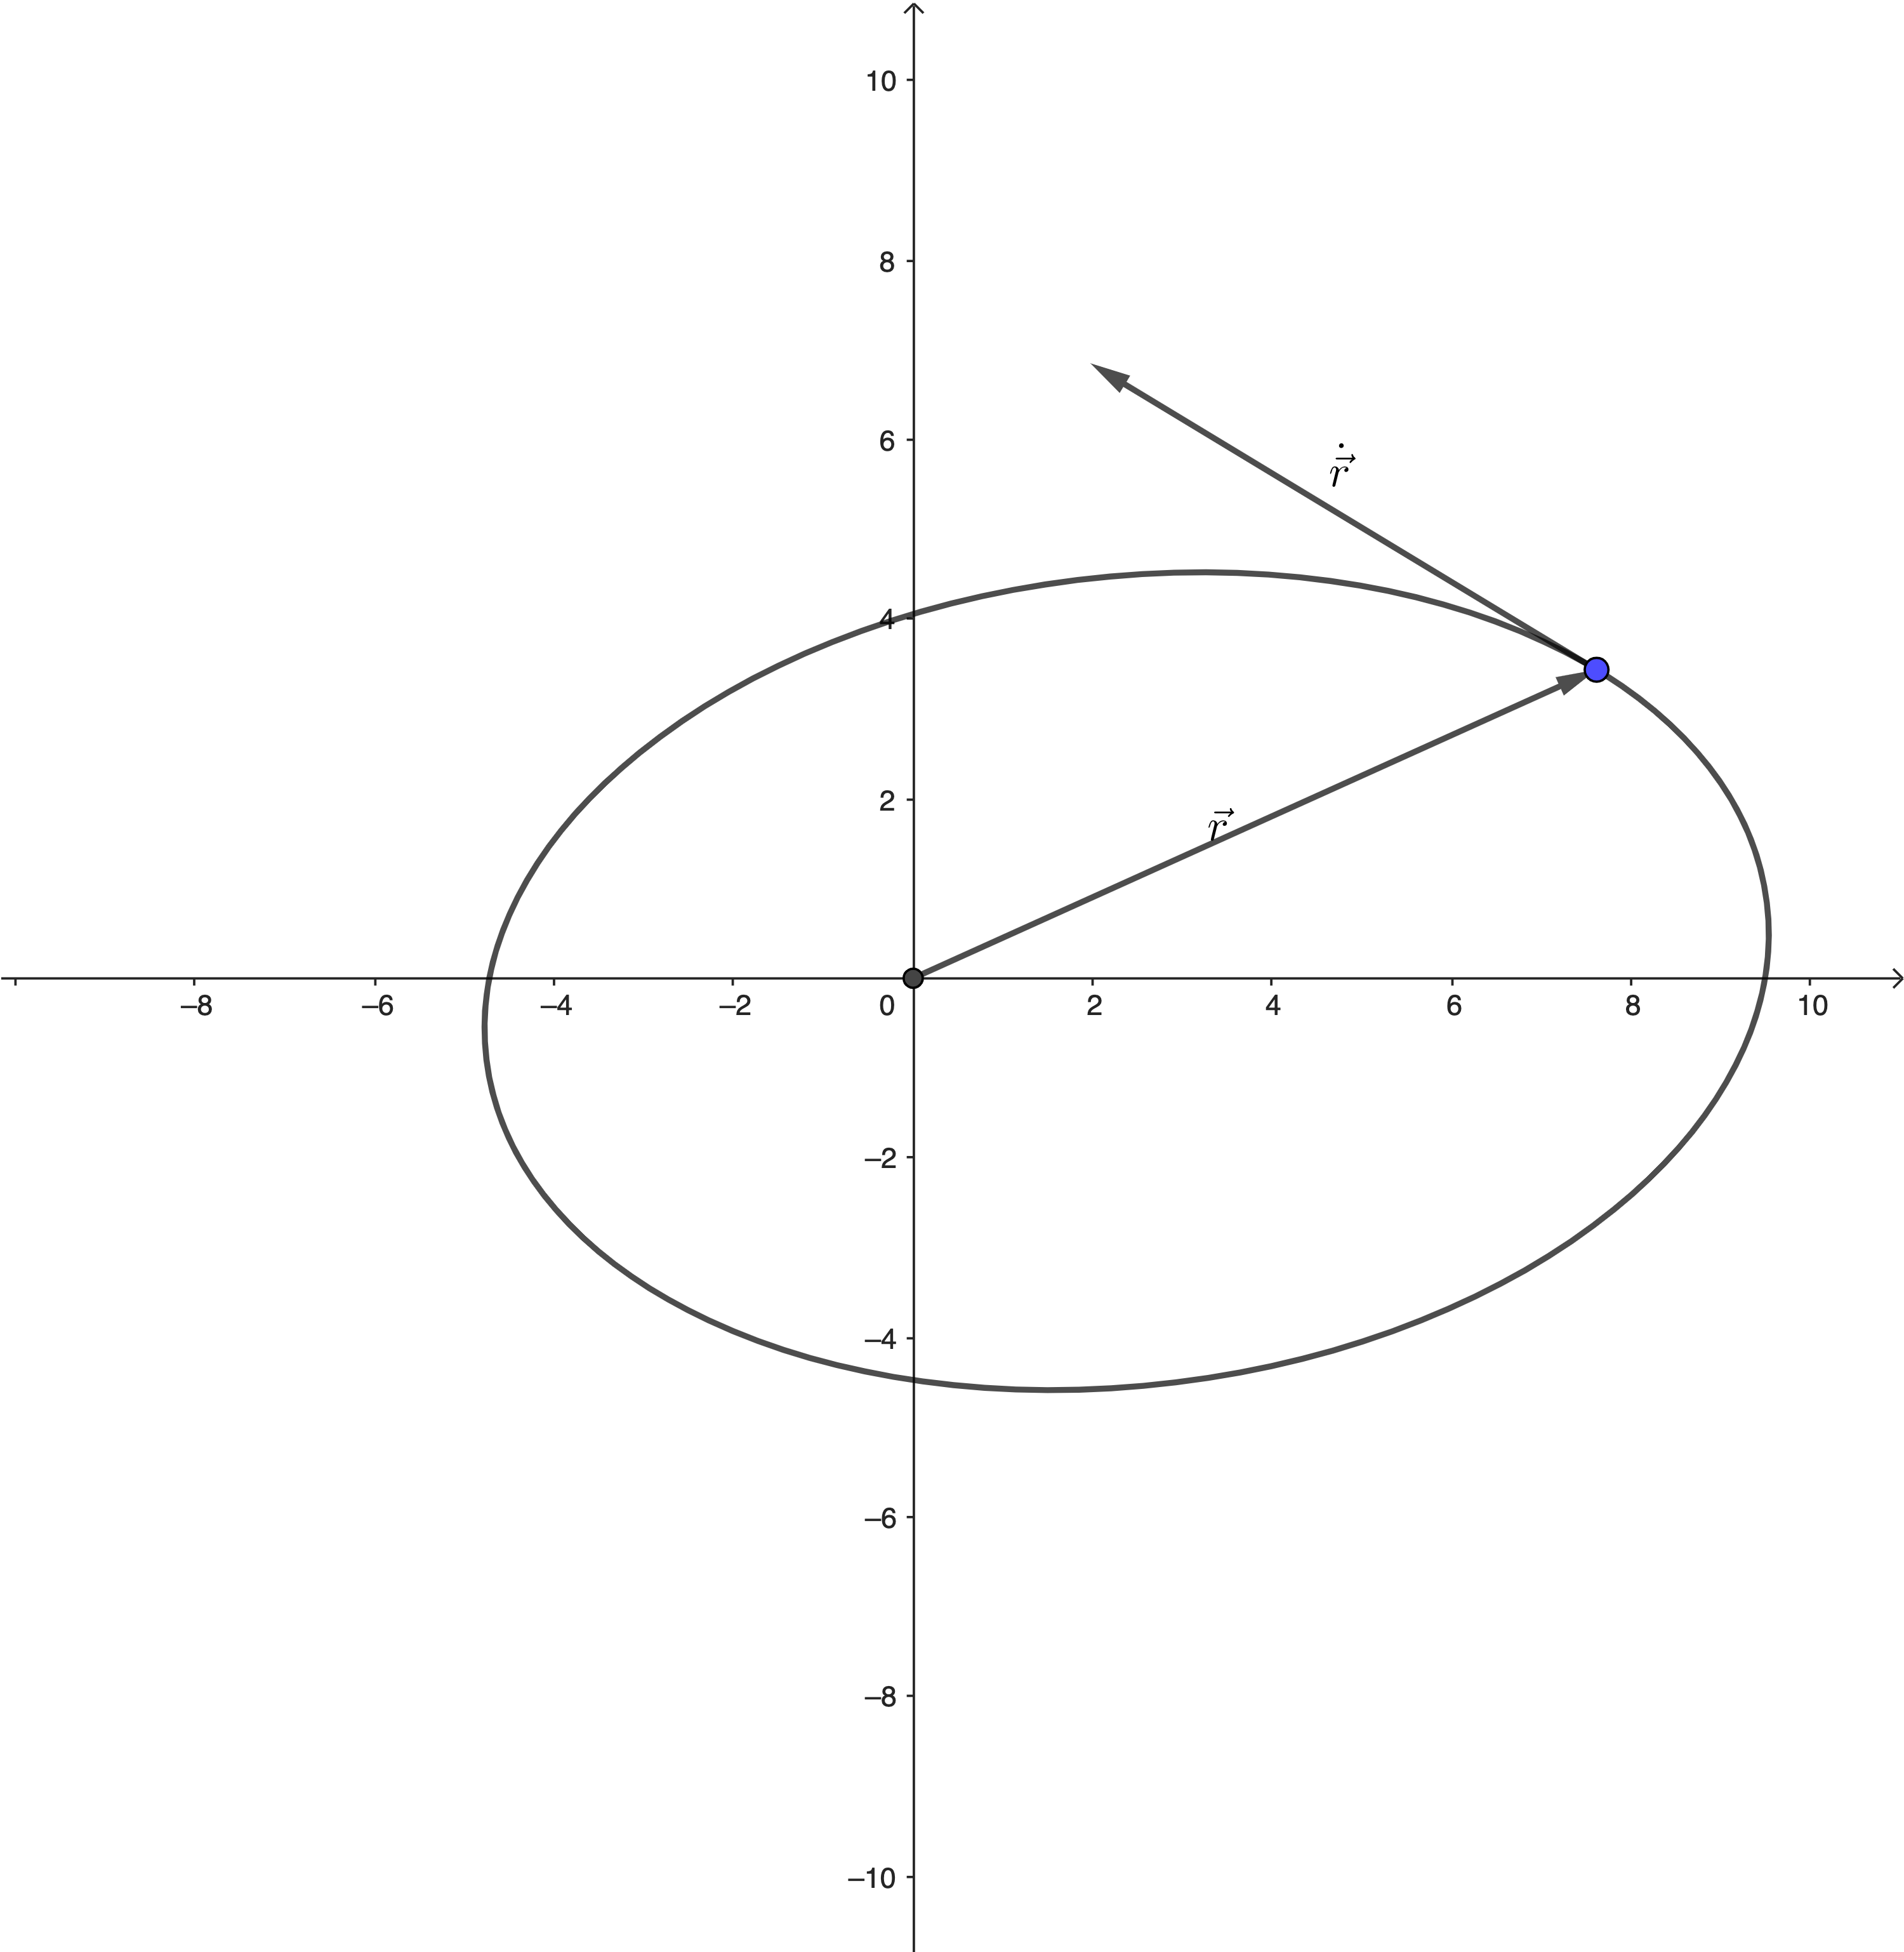
\includegraphics[width = 0.5 \textwidth]{Tangentialvektor.png}
\end{center}
\clearpage

\begin{bsp}
    {Diskussion einer Parametrisierten Kurve}{}
    Gegeben ist die parametrisierte Kurve mit der Gleichung:
    $$ \vec{r}: [0, 2\pi] \to \R^2, \quad \vec{r}(t) = \begin{pmatrix}
        1-\sin(2t) \\ 
        \cos(t)
    \end{pmatrix}$$
    Bestimme die Achsenschnittpunkte und die Kurvenpunkte mit Tangenten parallel zu den Koordinatenachsen. Skizziere anschliessend die Kurve.

    \vspace*{18 cm}

\end{bsp}

\clearpage
\begin{ueb}
    {}{}

\begin{enumerate}
    \item Kreise
    \begin{enumerate}
        \item Betrachten Sie die Parameterdarstellung eines Kreises mit Radius 1: $$\vec{r}(t) = \begin{pmatrix}
            \cos(t) \\ \sin(t)
        \end{pmatrix} , \quad t \in [0, 2\pi] $$
        Zeigen Sie mit dem Skalarprodukt, dass $\dot{\vec{r}} (t)$ und $\vec{r}(t)$ senkrecht aufeinander stehen.

        In welche Richtung zeigt $\ddot {\vec{r}}$ ?
        \item Betrachten Sie eine alternative Parametergleichung für den Kreis:
        $$\vec{r}_2(t) = \begin{pmatrix}
            \cos(2t) \\ \sin(2t)
        \end{pmatrix} , t \in [0, \pi] $$
        Vergleichen Sie $\dot{\vec{r_2}} (t)$ mit $\dot {\vec{r}} (t)$ aus Aufgabe (a). Interpretation?
    \end{enumerate}


    \item Die folgenden Kurven sind in Parameterdarstellung gegeben. Bestimmen Sie rechnerisch die Schnittpunkte mit den Koordinatenachsen und die Kurvenpunkte mit Tangenten parallel zu den Koordinatenachsen. Zeichnen Sie diese Kurven mit Geogebra und überprüfen Sie damit Ihre Lösungen.

    \begin{enumerate}
        \item \(\begin{pmatrix}
            x \\
            y
        \end{pmatrix} = \begin{pmatrix}
            t \\
            2t^2 + t - 1
        \end{pmatrix}\)
    
        \item \(\begin{pmatrix}
            x \\
            y
        \end{pmatrix} = \begin{pmatrix}
            t^2 - 1 \\
            t^3 - t
        \end{pmatrix}\)
    
        \item \(\begin{pmatrix}
            x \\
            y
        \end{pmatrix} = \begin{pmatrix}
            \sin 2t \\
            \cos t
        \end{pmatrix}\)
    
        \item \(\begin{pmatrix}
            x \\
            y
        \end{pmatrix} = \begin{pmatrix}
            2\sqrt{2 + t} \\
            \sqrt{2 - t}
        \end{pmatrix}\)
    
        \item \(\begin{pmatrix}
            x \\
            y
        \end{pmatrix} = \begin{pmatrix}
            t - \sin t \\
            1 - \cos t
        \end{pmatrix}\)
    
        \item \(\begin{pmatrix}
            x \\
            y
        \end{pmatrix} = \begin{pmatrix}
            1 + \sin t \\
            2 \cos 2t
        \end{pmatrix}\)
    
        % \item \(\begin{pmatrix}
        %     x \\
        %     y
        % \end{pmatrix} = \begin{pmatrix}
        %     t - \sin t \\
        %     t - \cos t
        % \end{pmatrix}\)
    
        \item \(\begin{pmatrix}
            x \\
            y
        \end{pmatrix} = \begin{pmatrix}
            \sinh t \\
            \cosh t
        \end{pmatrix} = \frac{1}{2}\begin{pmatrix}
            e^t - e^{-t} \\ 
            e^t + e^{-t}
        \end{pmatrix}\)
    \end{enumerate}
\end{enumerate}
    
\end{ueb}

\clearpage
\emph{Lösungen}
\begin{enumerate}
    \item Easy :) 
    \item 
\begin{enumerate}
    \item Parabel:
    
    Achsenschnittpunkte $ \left(-1, 0\right), \left(\frac{1}{2}, 0\right), \left(0, -1\right)$. 
    
    Tangenten parallel zur $x$-Achse: $ \left(-\frac{1}{4}, -\frac{9}{8}\right)$. 

    Tangenten parallel zur $y$-Achse: Keine.

    \item ``Parabola nodata''
    
    Achsenschnittpunkte $ \left(-1, 0\right), \left(0, 0\right)$. 
    
    Tangenten parallel zur $x$-Achse: $ \left(-\frac{2}{3}, \pm\frac{2\sqrt{3}}{9}\right)$. 

    Tangenten parallel zur $y$-Achse: $\left(-1, 0\right)$


    \item Achsenschnittpunkte $ \left(0, 0\right), \left(0, \pm 1\right)$. 
    
    Tangenten parallel zur $x$-Achse: $ \left(0, \pm 1\right)$. 

    Tangenten parallel zur $y$-Achse: $\left(\pm1, \pm\frac{\sqrt{2}}{2}\right)$

    \item Achsenschnittpunkte $ \left(4, 0\right), \left(0, 2\right)$. 
    
    Tangenten parallel zur $x$-Achse: keine. 

    Tangenten parallel zur $y$-Achse: keine.

    \item Achsenschnittpunkte $ \left(2k\pi, 0\right)$. 
    
    Tangenten parallel zur $x$-Achse:  $ \left((2k+1)\pi, 2\right)$. 

    Tangenten parallel zur $y$-Achse: keine.
    
    \item ``Zykloide''
    
    Achsenschnittpunkte $ \left(1\pm\frac{\sqrt{2}}{2}, 0\right), \left(0, -2\right)$. 
    
    Tangenten parallel zur $x$-Achse: $ \left(1, 2\right)$. 

    Tangenten parallel zur $y$-Achse: keine.

    \item Hyperbel
    
    Achsenschnittpunkte $ \left(0, 1\right)$. 
    
    Tangenten parallel zur $x$-Achse: $ \left(0, 1\right)$.

    Tangenten parallel zur $y$-Achse: keine.



    
\end{enumerate}
\end{enumerate}




